\section*{Problema 5}

\textbf{En este ejercicio usamos intervalos de confianza para entender mejor el desempeño de algoritmos. En general, el componente aleatorio puede entrar de dos maneras: en la dinámica del algoritmo o por los datos/parámetros de entrada. Calcula un intervalo de confianza de 95\% para el promedio del tiempoque los algoritmos quicksort y shellsort requieren para ordenar 10,000,000 números elegidos al azar de una distribución continua, basado en 100 corridas de cada algoritmo. Puedes usar la versión que está en R. Por ejemplo, para calcular el tiempode una corrida el código es:}

\begin{verbatim}
    system.time(x1 <- sort(x, method = "shell"), gcFirst = TRUE)[1]
    system.time(x2 <- sort(x, method = "quick"), gcFirst = TRUE)[1]
\end{verbatim}

\textbf{con GcFirst = FIRST se libera primero la memoria (en caso de que sea
    posible) Explica porque no importa de cual distribución se generan los números siempre y cuando que sean de una variable continua. Construye también un intervalo de confianza para la diferencia de sus tiempos de ejecución para un (mismo) conjunto.}

La razón por la cual no importa la elección de la distribución es debido a que los algoritmo de ordenamiento realizaran una función semejante independientemente de la distribución de los números generados. Otra razón que podemos dar de esta invarianza es el teorema del límite central, ya que toda distribución continua con varianza no nula y fínita se aproximará a una distribución normal. Para este ejercicio se generaron $10,000,000$ números aleatorios usando una distribución uniforme ($X \sim \mathcal{U}(0,1)$). Se crearon 100 sets de la cantidad de números aleatorios y se ordenaron usando los algoritmos quick sort y shell sort. En la figura \ref{fig:time_sort} se representan las distribuciones del tiempo de ejecucción del algoritmo de quick sort (figura \ref{fig:quick_sort}) y shell sort (figura \ref{fig:shell_sort}).

\begin{figure}[H]
    \centering
    \begin{subfigure}[b]{8cm}
        \centering
        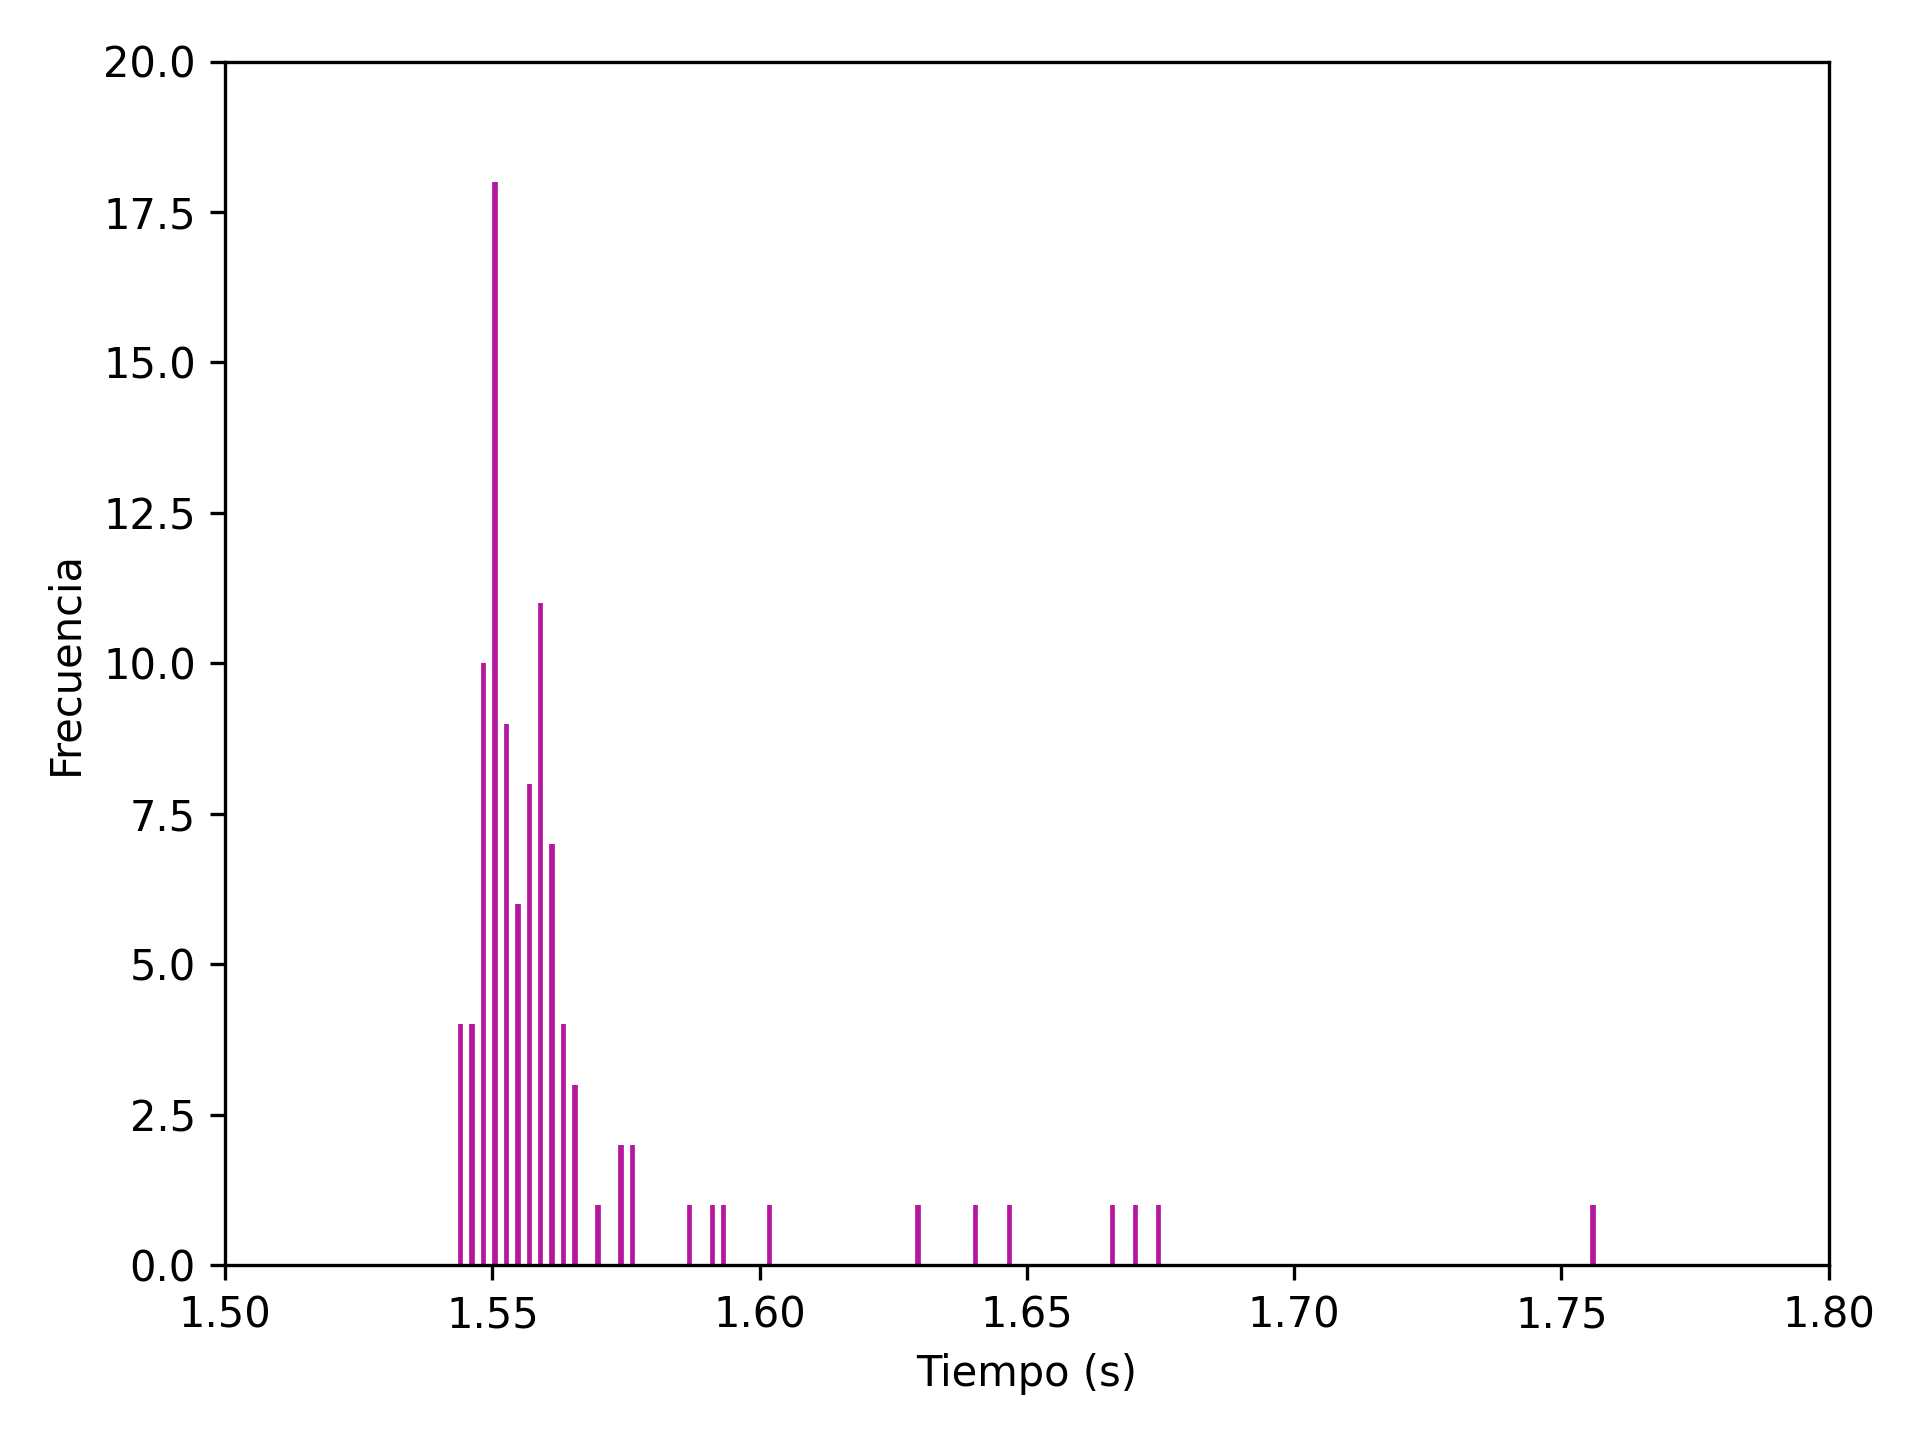
\includegraphics[width=8cm]{Graphics/quick_sort.png}
        \caption{Distribución del tiempo de ejecucción del algoritmo quick sort.}
        \label{fig:quick_sort}
    \end{subfigure}
    \hspace{0.5cm}
    \begin{subfigure}[b]{8cm}
        \centering
        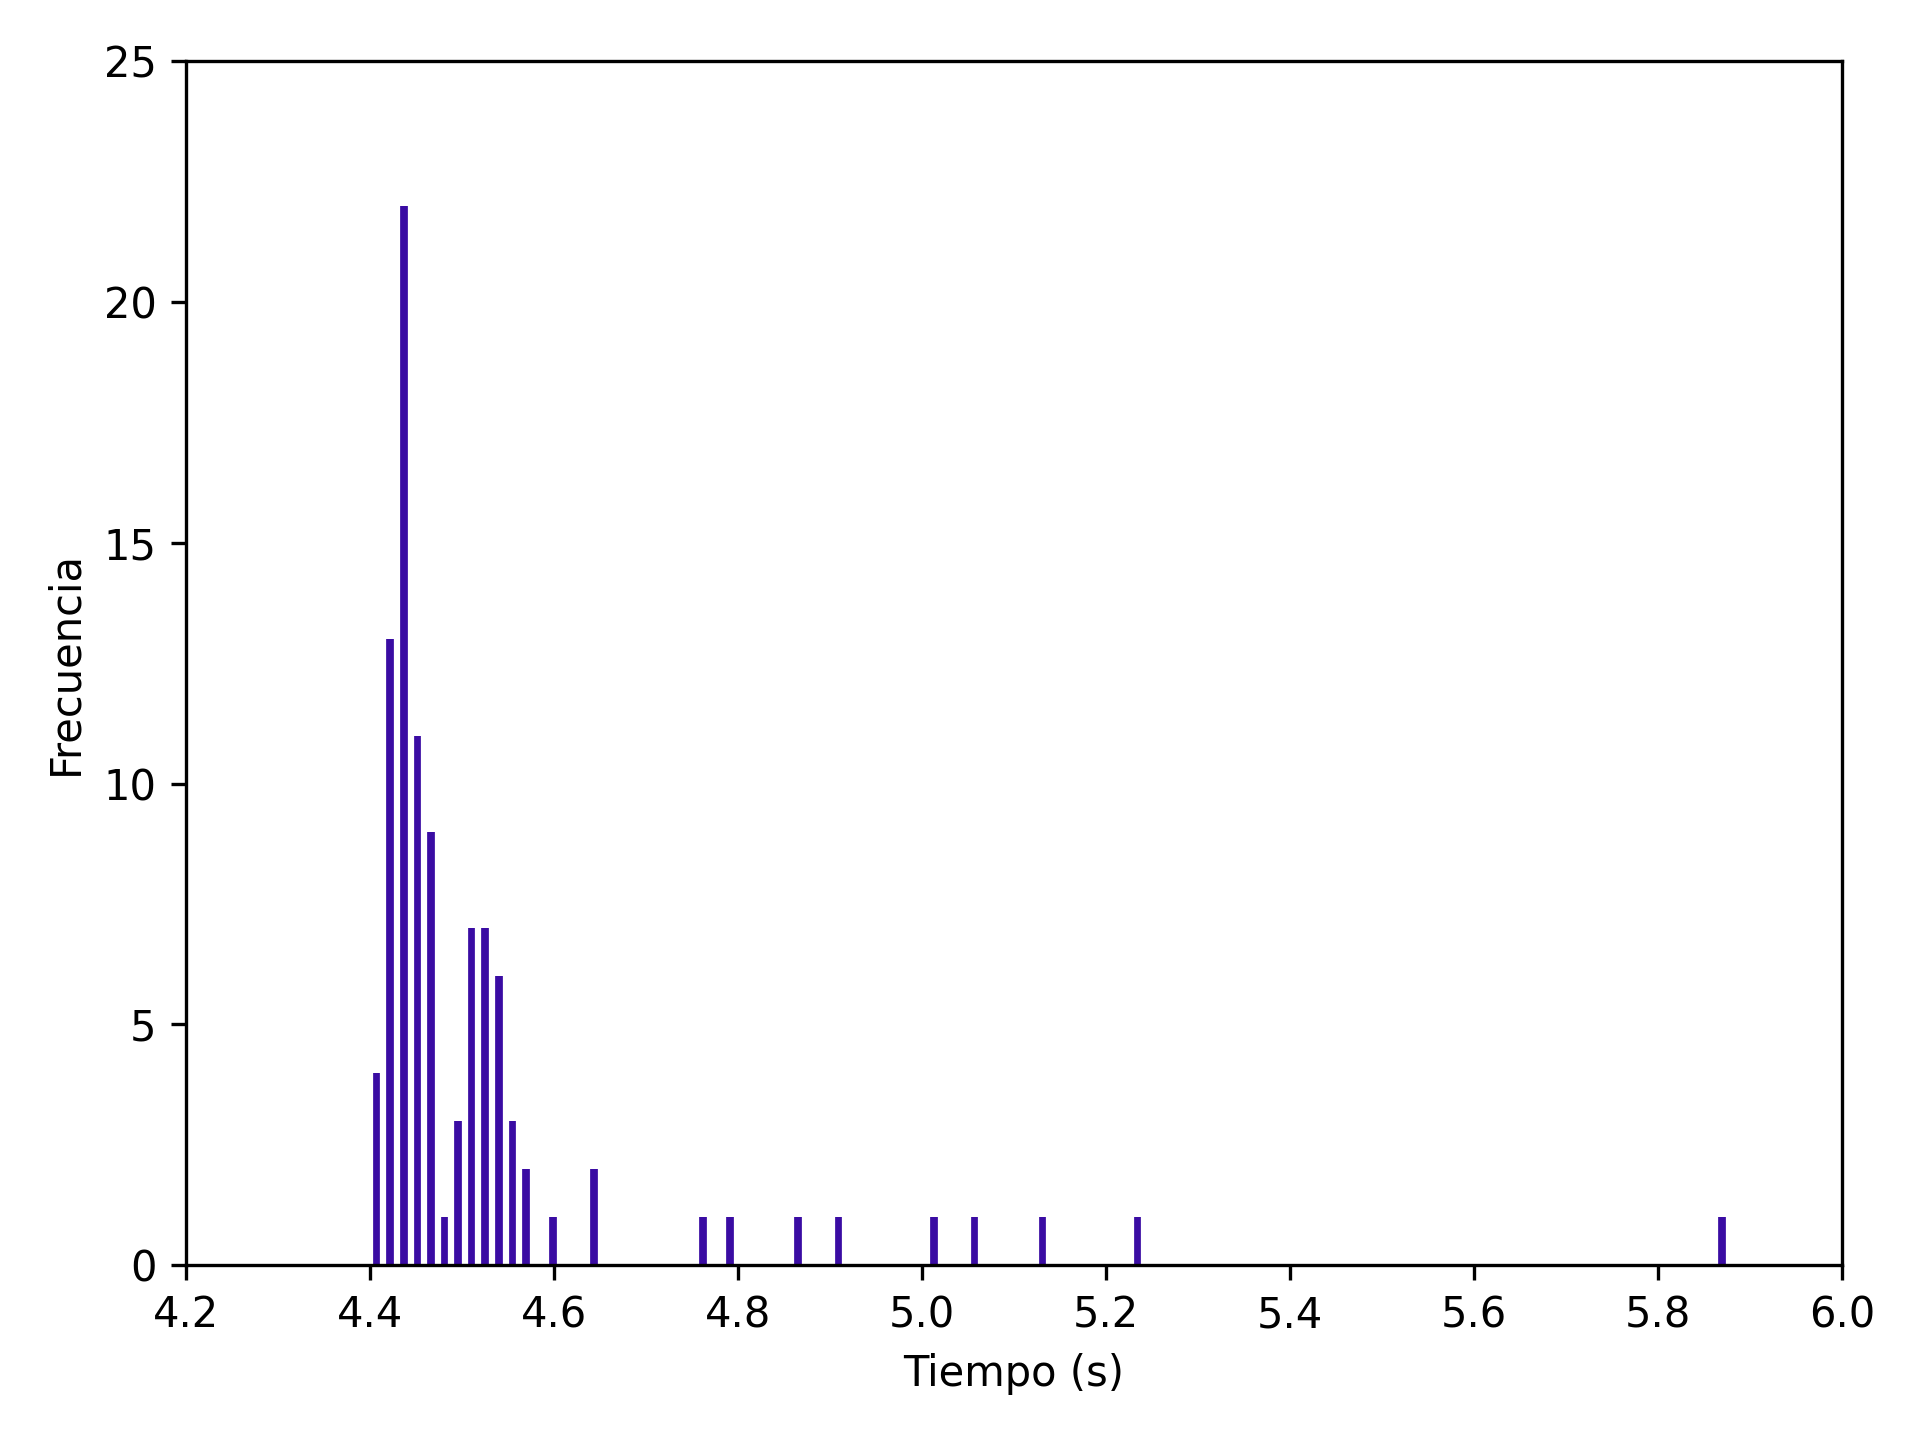
\includegraphics[width=8cm]{Graphics/shell_sort.png}
        \caption{Distribución del tiempo de ejecucción del algoritmo shell sort.}
        \label{fig:shell_sort}
    \end{subfigure}
    \caption{Distribuciones del tiempo de ejecución para los diferentes algoritmos de ordenamiento.}
    \label{fig:time_sort}
\end{figure}

Realizando la resta de los tiempos ejecución para un mismo set de datos generdos se obtuvo la distribución mostrada en la figura \ref{fig:diff_problema4}.

\begin{figure}[H]
    \centering
    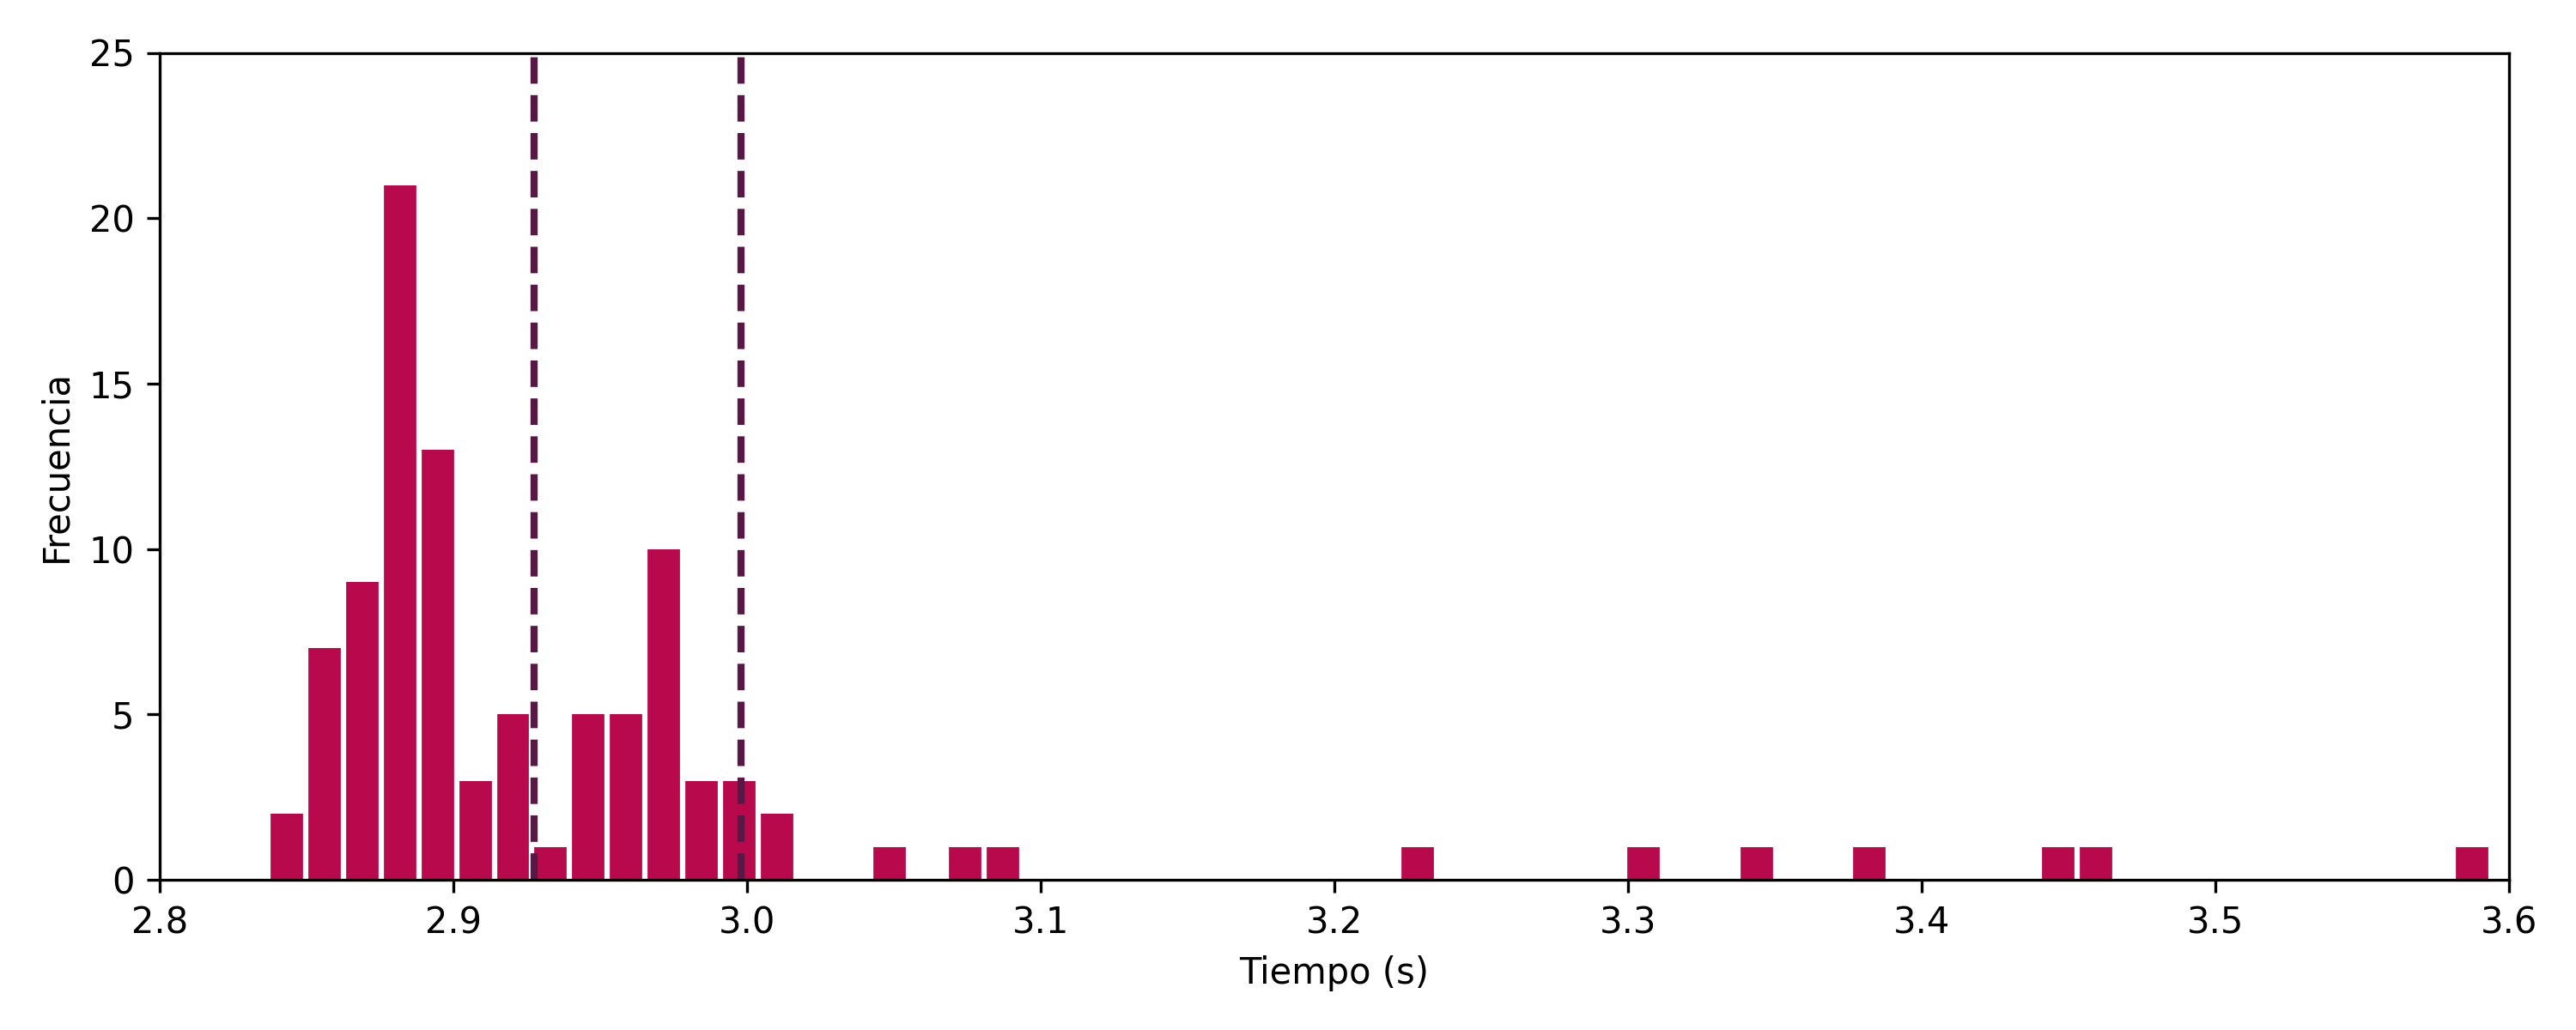
\includegraphics[width=13cm]{Graphics/diff.png}
    \caption{Distribución e intervalo de confianza de la diferencia en los tiempos de ejecución entre los algoritmos de ordenamiento. }
    \label{fig:diff_problema4}
\end{figure}

El promedio, la varianza y el intervalo de confianza obtenidos de estos datos se encuentran en la tabla \ref{table:datos}.

\begin{table}[H]
    \centering
    \begin{tabular}{ccc} \hline
        \textbf{Promedio} ($\mu$) & \textbf{Varianza} ($\sigma^2$) & \textbf{IC}         \\ \hline
        2.96273                   & 0.032194                       & [2.927563,2.997897] \\ \hline
    \end{tabular}
    \caption{Promedio, varianza e intervalo de confianza obtenidos de la diferencia en los tiempos de ejecucción.}
    \label{table:datos}
\end{table}

